\documentclass[12pt]{article}
\usepackage[utf8]{inputenc}
\usepackage[T2A]{fontenc}
\usepackage[mongolian]{babel}
\usepackage{graphicx}
\usepackage{amsmath}
\usepackage{amssymb}
\graphicspath{{images/}}
\title {Хичээлийн материал оруулах систем хөгжүүлэх}
\begin{document}
	\maketitle
	\section{Функциональ шаардлага}
		\subsection{Багшын шаардлага}
	\begin{itemize}
	
		\item Улирлаар хичээлээ үүсгэх
		\item Хичээлийн материал оруулах хичээлээ сонгох
		\item Хичээлийн материал болох .pdf болон .ppt өргөтгөлтэй файлаа оруулах
		\item Тухайн хичээлийг үзэж байгаа оюутнуудыг нэмэх
		
		
		
		\item Хайлт хийх
		
			\subsection{Оюутны шаардлага}
			\begin{itemize}
				\item Үүссэн хичээ рүү орох
				\item Хичээлийн материалаа систем дээр нээж харах болон татаж үзэх
			\end{itemize}
		
		\subsection{Системийн шаардлага}
		\begin{itemize}
			\item Тайлан гаргах
				\subitem Хамгийн их файл оруулдаг багш нарын тайланг графикаар харуулах
				\subitem Файлын тоог улирлаар харуулах
				\subitem Татагдсан файлын тоог харуулах
			\item Мэдэгдэл шидэх
		\end{itemize}
	\end{itemize}
	\section{Функциональ бус шаардлага}
		\begin{itemize}
			\item Бүтээгдэхүүний 
			\subitem Хичээлийн материалыг систем дээр харуулах
			\subitem Системийн цагийн хуваарь 24/7 байх
			\subitem Бүх төрлийн төхөөрөмжөөс үзэхэд тохиромжтой хэлбэрээр харагддаг байх буюу загвар нь responsive байх
			
			\item Байгууллагын
			\subitem Өгөгдлийн санд өгөгдлийг нэг форматаар хадгалагддаг байх
			
			\item Гадаад
			\subitem Системд нэвтрэх эрхийг хязгаарлаж, хамгаалдаг байх
			\subitem Бусад албан байгууллагатай хамтран ажилладаг байх
		\end{itemize}
	\section{Юзкейс диаграм}	
		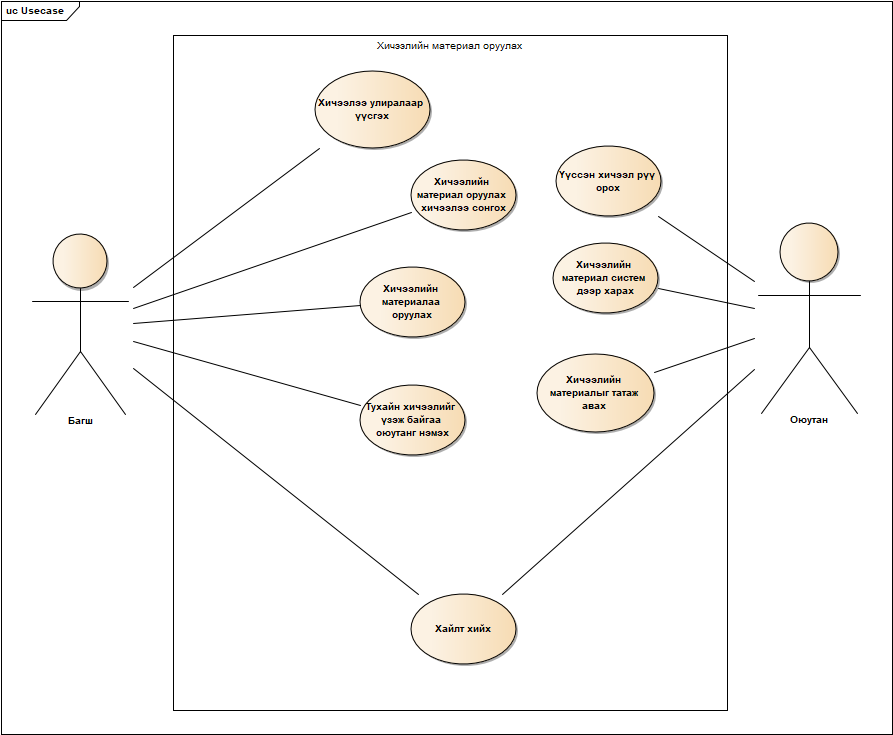
\includegraphics[scale=0.50]{usecase}
		
	\section{ERD диаграм}
		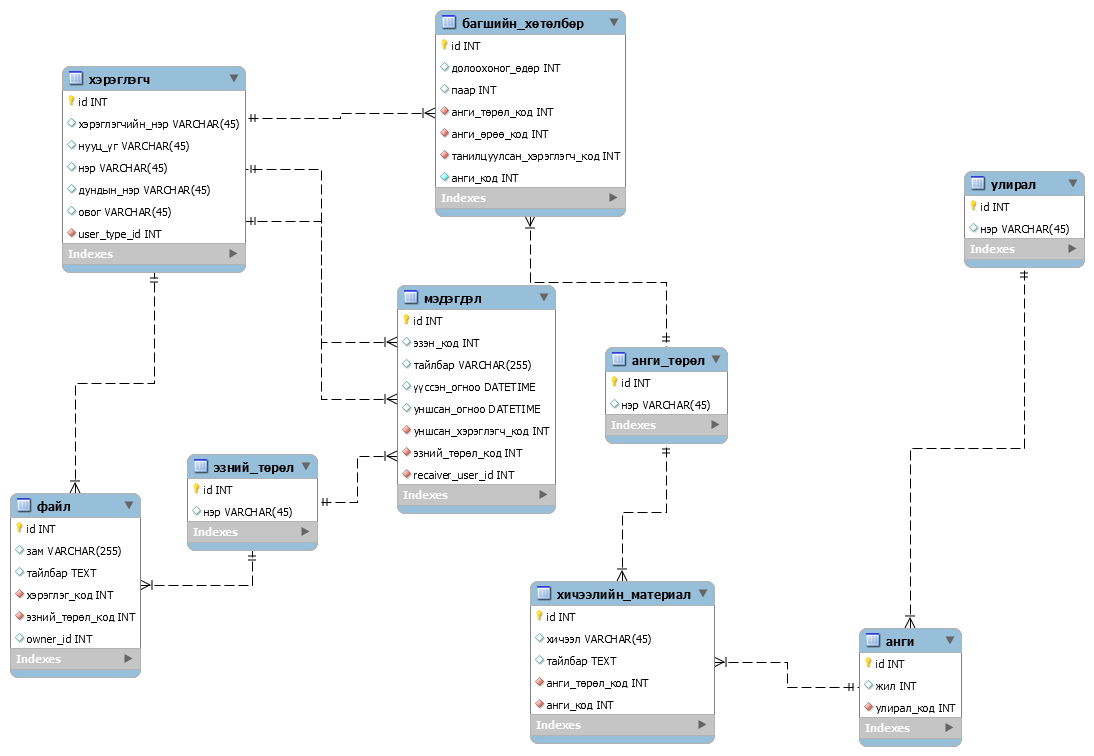
\includegraphics[scale=0.5]{ERD}
		
	\section{Оюутан хичээлийн материал харах болон даалгавар илгээх үйл ажиллагааны диаграм}
		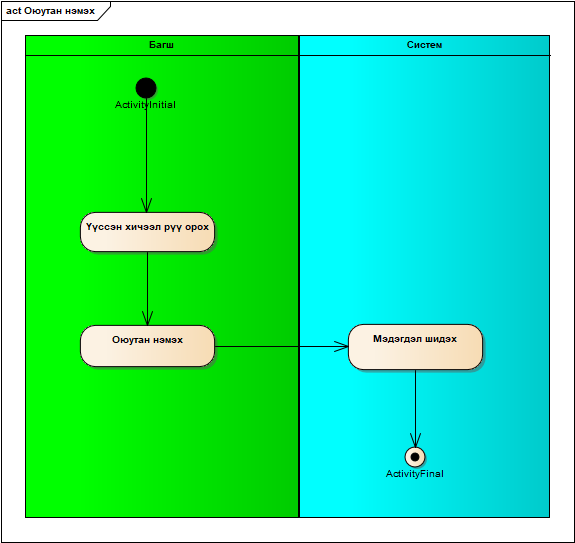
\includegraphics[scale=0.8]{activity}
	
	\section{Багш хичээлийн материал оруулах үйл ажиллагааны диаграм}
		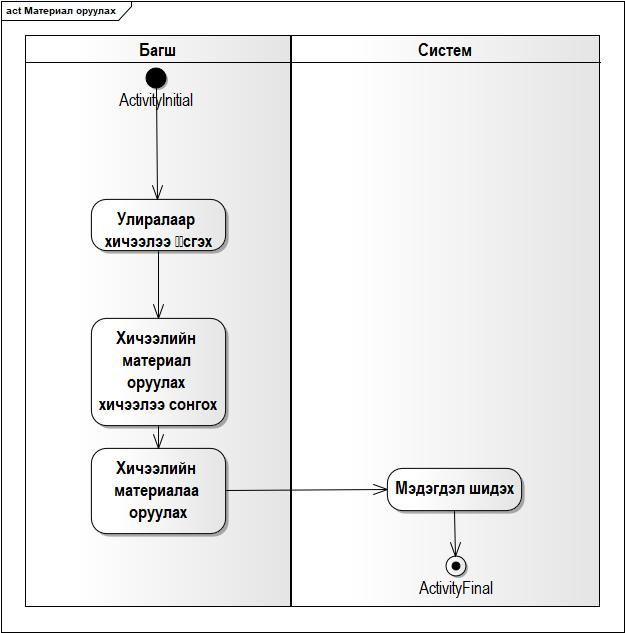
\includegraphics[scale=0.8]{activity1}
		
	\section{Класс диаграм}
		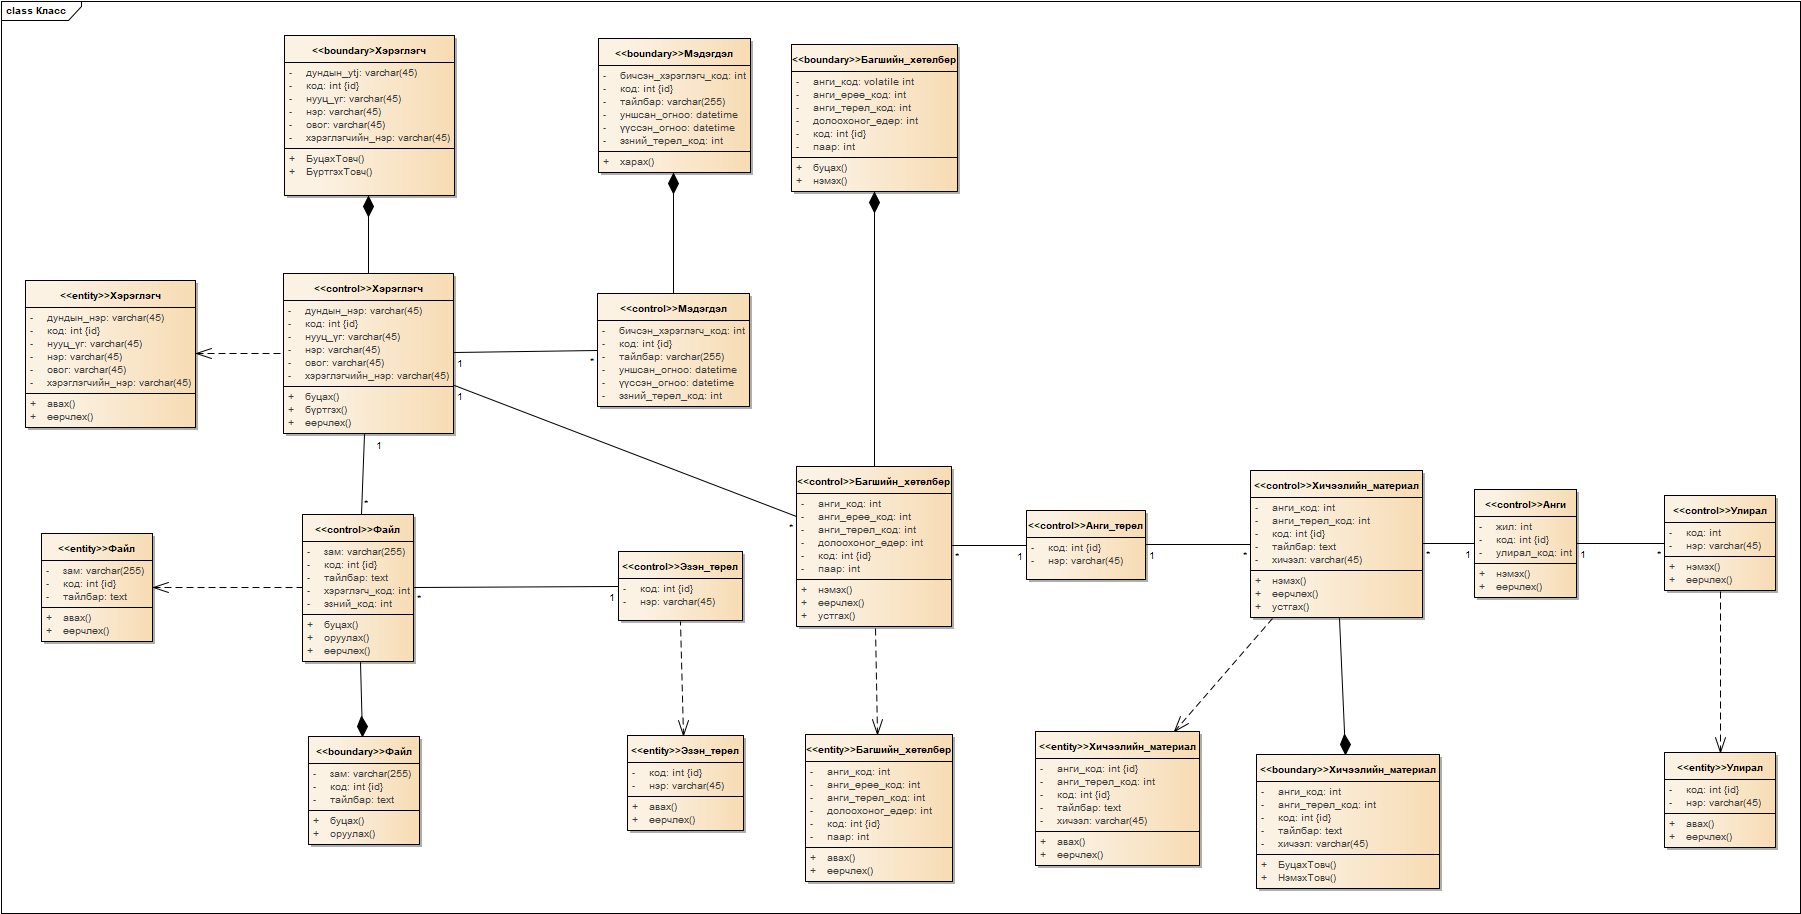
\includegraphics[scale=0.5]{Class} 
		
	\section{Багшын системд хийх үйлдлийн дарааллын диаграм}
		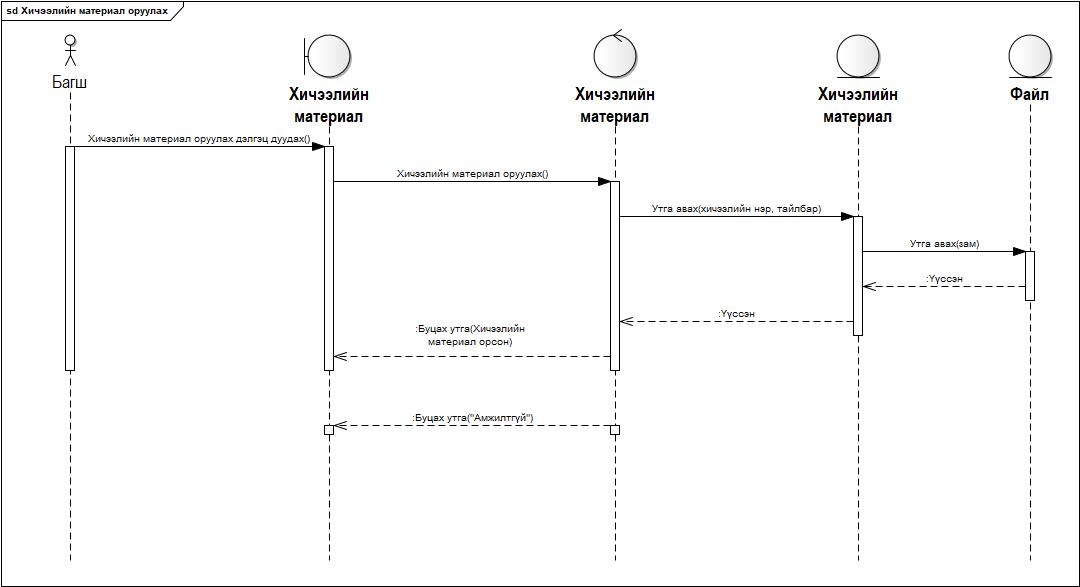
\includegraphics[scale=0.4]{sequence1}
		
	\section{Оюутны системд хийх үйлдлийн дарааллын диаграм}
		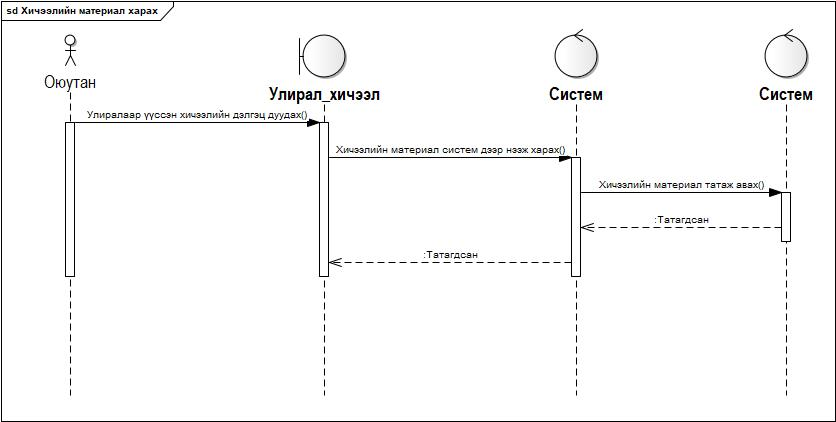
\includegraphics[scale=0.4]{sequence2}
	
	
	
\end{document}